%!TEX root = ../thesis.tex
\chapter{Аналіз застосування GAN для аугментації навчальних вибірок}
\label{chap:practice}

У даному розділі ми застосуємо розглянуті нами у попередніх
частинах моделі та методи на практиці, а саме навчимо варіацію
моделі архітектури UNet з різними функціями помилки. Обрахуємо
метрики і визначимо чи дійсно проблема незбалансованості
класів істотно впливає на якість семантичної сегментації супутникових
знімків. І на сам кінець за допомогою генеративно-змагальних
мереж згенеруємо штучні приклади, які додамо до реальних даних
та будемо проводити навчання вже на ції аугментованій вибірці.
І визначимо чи дійсно подібний спосіб дозволяє
покращити якість семантичної сегментації.

Вихідний код, який був створено для усіх наведених у даному
розділі експериментів доступний на GitHub
\footnote{\href{https://github.com/ShkalikovOleh/SatelliteGAN}
    {https://github.com/ShkalikovOleh/SatelliteGAN}}.

\section{Попередня обробка навчальних даних}

Для перевірки того, чи дійсно запропонований підхід
дозволить збільшити якість семантичної сегментації супутникових знімків
проведемо експерименти з класифікації на 19 класів
композиту Sentinel-2A \cite{drusch2012sentinel}
для Київської області взятих з 1 липня по 1 серпня 2021 року.
Класи представляють собою здебільшого сільськогосподарські
культури, тому розв'язання задачі сегментації саме на таких
даних має широкий прикладний потенціал.

Ми використовували саме композит супутникових знімків, бо
територія Київської області надто велика, щоб вона могла
повністю розміститися на одному супутниковому знімку Sentinel-2A.
Саме тому був взятий часовий ряд червоного, зеленого, синього та
ближнього інфрачервоного каналів за липень 2021~р., який потім був об'єднаний.
У тих частинах, що перетиналися були, були обрані медіанні значення
пікселів, також знімки були очищені від детектованих хмар та тіней від них.

Після чого ці дана колекція знімків була об'єднана у один
великий композит для Київської області та до цього композиту
була додана окремим каналом маска з мітками класів, яка була
отримана у результаті досліджень науковцями інституту
космічних досліджень Національної академії наук України.

Сучасні нейромережеві архітектури не дозволяють нам працювати
з зображення дуже великого розміру, тому ми вимушені
розрізати отриманий композит на квадратні частини розміром $256 \times 256$
пікселів. Такий вибір обґрунтований тим, що саме такий розмір
зображення генерувався авторами класичного Pix2Pix  \cite{pix2pix}.

Попри те, що ми брали дані за місяць, все одно залишились
території, які не були покриті супутником за спостережуваний період.
До того ж, контури Київської області не є ідеальною геометричною фігурою,
тож на деяких знімках, на яких показані кордони області відсутні значення
пікселів або масок, які відповідають іншим областям.
Через ці два фактори у деяких отриманих зображеннях
присутні пікселі, у яких відсутнє значення.
Такі приклади були відфільтровані та не
використовувалися при навчанні нейронних мереж.

На сам кінець, через те, що використовувалися знімки з
попередньою обробкою та корекцією класу TOA, то
область значень кожного з каналів була не класичною
$[0, 1]$, а мала більше максимальне значення.
У свою чергу більшість нейромережевих архітектур працює зі
значеннями у проміжку $[-1, 1]$.
Тож був застосований аналог min-max нормалізації, а саме
кожне значення пікселю кожного каналу було поділено на
максимальне значення для даного каналу даного зображення,
а після цього класична стандартизація з математичним
сподівання і стандартним відхиленням рівними $0.5$.

\section{Результати сегментації без використання GAN}

Для розв'язання задачі семантичної сегментації
даної вибірки супутникових знімків було використано
архітектуру UNet. Для того, щоб ми мали змогу перевірити
якість моделі використовуючи метрики, і при цьому
отримали достовірні значення, тобто уникнули явища
перенавчання, вибірку було поділено навпіл на навчальну і тестову.

У якості енкодера у використаній варіації UNet було обрано
ResNet-34, що є компромісом між обчислювальною потужністю,
необхідною для навчання подібних моделей та
складністю мережі.

Дана вибірка є незбалансованою, що можна побачити на
статистиках по сумарній кількості пікселів
для кожного класів на рис. \ref{fig:pixels_per_class}
(мітки класів відповідають назвам, які можна знайти
у таблиці \ref{tab:segm_result_real_per_classes}).
Тож для подолання проблем, які пов'язані з цим, ми спробували
застосувати різні функції помилок, а саме зважені та
не зважені Cross-Entropy
та Focal Loss. У якості вагових коефіцієнтів для кожного
класу були обрані зворотні відношення сумарної кількості пікселів класу
до кількості усіх пікселів у тренувальній вибірці.

У якості оптимізатора було обрано добре відомий,
один з найбільш застосовуваних та ефективних,
алгоритм Adam \cite{kingma2014adam} зі швидкістю навчання
$2 \cdot 10^{-4}$. Розмір батчу дорівнював $64$.

\begin{table}[!ht]
    \centering
    \caption{Глобальні метрики точності сегментації
        для реальної вибірки}
    \begin{tabular}{|c|C|C|C|C|}
        \hline
        \multirow{2}{*}{Метрика} & \multicolumn{2}{c|}{CE Loss} & \multicolumn{2}{c|}{Focal Loss}             \\
        \cline{2-5}              & w/o W                        & W                               & w/o W & W \\
        \hline $\acc$            & 89                           & 79                              & 4     & 4 \\
        \hline $\varkappa$       & 69                           & 0.715                           & 4     & 4 \\
        \hline $\iou$            & 89                           & 79                              & 4     & 4 \\
        \hline
    \end{tabular}
    \label{tab:segm_result_real_global}
\end{table}

У результаті $500$-та епох навчання було отримані значення
метрик, таких як точність ($\acc$), міра Жаккара ($\iou$) та
каппа Коена ($\varkappa$), для різних варіацій функції помилки.
Вони наведені у таблиці \ref{tab:segm_result_real_global}.

Що стосується якості сегментації за кожним з класів, то
слід звернутися до таких метрик як Producer Accuracy $\pracc$
та User Accuracy $\usacc$, наведених у таблиці \ref{tab:segm_result_real_per_classes}.

\begin{table}[!ht]
    \centering
    \caption{Метрики точності сегментації за класами
        для реальної вибірки}
    \begin{tabular}{|K|C|C|C|C|C|C|C|C|}
        \hline
        \multirow{3}{*}{Назва класу}   & \multicolumn{4}{c|}{UA}         & \multicolumn{4}{c|}{PA}                                             \\
        \cline{2-9}
                                       & \multicolumn{2}{c|}{CE Loss}    & \multicolumn{2}{c|}{Focal Loss} &
        \multicolumn{2}{c|}{CE Loss}   & \multicolumn{2}{c|}{Focal Loss}                                                                       \\
        \cline{2-9}
                                       & w/o W                           & W                               & w/o W & W & w/o W & W & w/o W & W \\
        \hline Штучні об'єкти          & 69                              & 0.715                           & 4     & 4 & 4     & 4 & 4     & 4 \\
        \hline Зернові культури        & 89                              & 79                              & 4     & 4 & 4     & 4 & 4     & 4 \\
        \hline Ріпак                   & 0                               & 53                              & 4     & 4 & 4     & 4 & 4     & 4 \\
        \hline Гречка                  & 0                               & 0                               & 4     & 4 & 4     & 4 & 4     & 4 \\
        \hline Кукурудза               & 94                              & 87                              & 4     & 4 & 4     & 4 & 4     & 4 \\
        \hline Буряк                   & 0                               & 23                              & 4     & 4 & 4     & 4 & 4     & 4 \\
        \hline Соняшник                & 89                              & 94                              & 4     & 4 & 4     & 4 & 4     & 4 \\
        \hline Соя                     & 27                              & 66                              & 4     & 4 & 4     & 4 & 4     & 4 \\
        \hline Інші культури           & 0                               & 6                               & 4     & 4 & 4     & 4 & 4     & 4 \\
        \hline Ліс                     & 93                              & 93                              & 4     & 4 & 4     & 4 & 4     & 4 \\
        \hline Необроблювані землі     & 71                              & 76                              & 4     & 4 & 4     & 4 & 4     & 4 \\
        \hline Відкритий ґрунт         & 3                               & 54                              & 4     & 4 & 4     & 4 & 4     & 4 \\
        \hline Вода                    & 97                              & 97                              & 4     & 4 & 4     & 4 & 4     & 4 \\
        \hline Болото                  & 27                              & 34                              & 4     & 4 & 4     & 4 & 4     & 4 \\
        \hline Ячмінь                  & 5                               & 21                              & 4     & 4 & 4     & 4 & 4     & 4 \\
        \hline Горох                   & 0                               & 1                               & 4     & 4 & 4     & 4 & 4     & 4 \\
        \hline Трави                   & 0                               & 0                               & 4     & 4 & 4     & 4 & 4     & 4 \\
        \hline Сади, парки, лісополоси & 45                              & 50                              & 4     & 4 & 4     & 4 & 4     & 4 \\
        \hline Виноградники            & 0                               & 0                               & 4     & 4 & 4     & 4 & 4     & 4 \\
        \hline
    \end{tabular}
    \label{tab:segm_result_real_per_classes}
\end{table}

Як можна побачити,

\section{Результати сегментації з використанням аугментованого набору даних}

\subsection{Генерація доповнених вибірок}

Test

\begin{figure}[ht]
    \centering
    \includegraphics[width=\textwidth]{gen_examples_4.png}
    \caption{Архітектура Pix2Pix у застосуванні до супутникових знімків}
    \label{fig:gen_examples}
\end{figure}

\begin{figure}[ht]
    \centering
    \includegraphics[width=\textwidth]{real_examples_4.png}
    \caption{Архітектура Pix2Pix у застосуванні до супутникових знімків}
    \label{fig:real_examples}
\end{figure}

\begin{figure}[ht!]
    \centering
    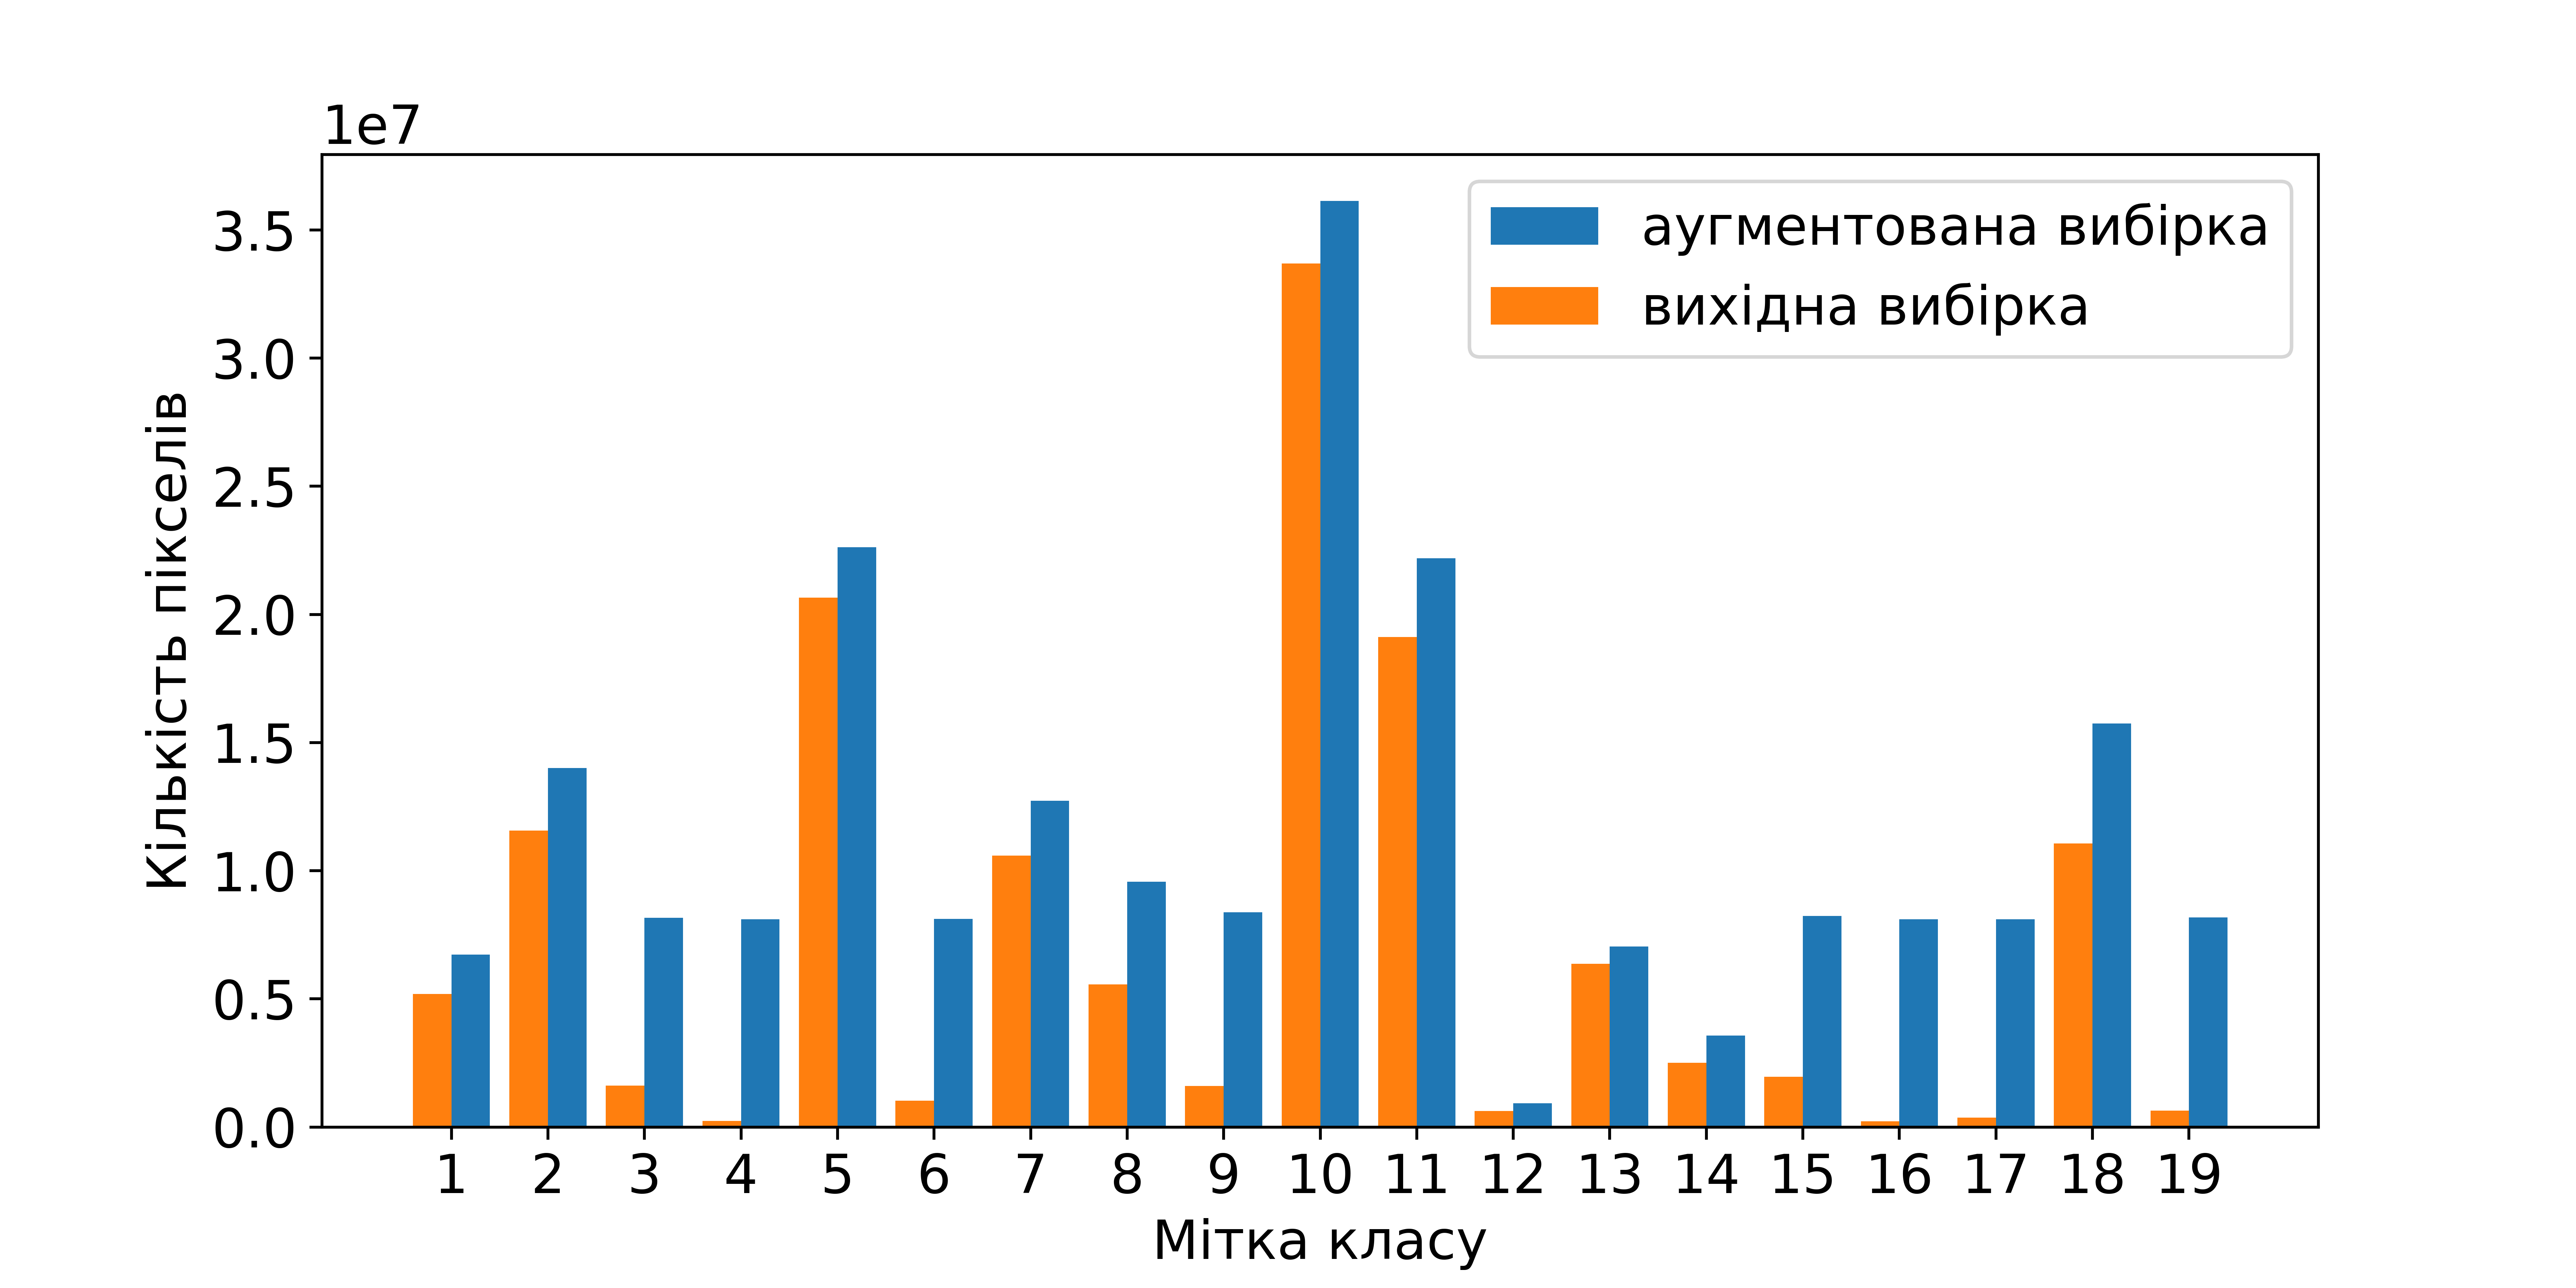
\includegraphics[scale=0.65]{dist_aug_real.png}
    \caption{Порівняння кількості пікселів для різних класів
        у досліджуваному та аугментованому наборах даних}
    \label{fig:pixels_per_class_aug}
\end{figure}

\subsection{Аналіз якості семантичної сегментації при застосуванні
    доповнених вибірок}

\begin{table}[!ht]
    \centering
    \caption{Глобальні метрики точності сегментації
        для реальної вибірки}
    \begin{tabular}{|c|C|C|C|C|}
        \hline
        \multirow{2}{*}{Метрика} & \multicolumn{2}{c|}{CE Loss} & \multicolumn{2}{c|}{Focal Loss}             \\
        \cline{2-5}              & w/o W                        & W                               & w/o W & W \\
        \hline $\acc$            & 89                           & 79                              & 4     & 4 \\
        \hline $\varkappa$       & 69                           & 0.715                           & 4     & 4 \\
        \hline $\iou$            & 89                           & 79                              & 4     & 4 \\
        \hline
    \end{tabular}
    \label{tab:segm_result_aug_global}
\end{table}

\begin{table}[!ht]
    \centering
    \caption{Метрики точності сегментації за класами
        для реальної вибірки}
    \begin{tabular}{|K|C|C|C|C|C|C|C|C|}
        \hline
        \multirow{3}{*}{Назва класу}   & \multicolumn{4}{c|}{UA}         & \multicolumn{4}{c|}{PA}                                             \\
        \cline{2-9}
                                       & \multicolumn{2}{c|}{CE Loss}    & \multicolumn{2}{c|}{Focal Loss} &
        \multicolumn{2}{c|}{CE Loss}   & \multicolumn{2}{c|}{Focal Loss}                                                                       \\
        \cline{2-9}
                                       & w/o W                           & W                               & w/o W & W & w/o W & W & w/o W & W \\
        \hline Штучні об'єкти          & 69                              & 0.715                           & 4     & 4 & 4     & 4 & 4     & 4 \\
        \hline Зернові культури        & 89                              & 79                              & 4     & 4 & 4     & 4 & 4     & 4 \\
        \hline Ріпак                   & 0                               & 53                              & 4     & 4 & 4     & 4 & 4     & 4 \\
        \hline Гречка                  & 0                               & 0                               & 4     & 4 & 4     & 4 & 4     & 4 \\
        \hline Кукурудза               & 94                              & 87                              & 4     & 4 & 4     & 4 & 4     & 4 \\
        \hline Буряк                   & 0                               & 23                              & 4     & 4 & 4     & 4 & 4     & 4 \\
        \hline Соняшник                & 89                              & 94                              & 4     & 4 & 4     & 4 & 4     & 4 \\
        \hline Соя                     & 27                              & 66                              & 4     & 4 & 4     & 4 & 4     & 4 \\
        \hline Інші культури           & 0                               & 6                               & 4     & 4 & 4     & 4 & 4     & 4 \\
        \hline Ліс                     & 93                              & 93                              & 4     & 4 & 4     & 4 & 4     & 4 \\
        \hline Необроблювані землі     & 71                              & 76                              & 4     & 4 & 4     & 4 & 4     & 4 \\
        \hline Відкритий ґрунт         & 3                               & 54                              & 4     & 4 & 4     & 4 & 4     & 4 \\
        \hline Вода                    & 97                              & 97                              & 4     & 4 & 4     & 4 & 4     & 4 \\
        \hline Болото                  & 27                              & 34                              & 4     & 4 & 4     & 4 & 4     & 4 \\
        \hline Ячмінь                  & 5                               & 21                              & 4     & 4 & 4     & 4 & 4     & 4 \\
        \hline Горох                   & 0                               & 1                               & 4     & 4 & 4     & 4 & 4     & 4 \\
        \hline Трави                   & 0                               & 0                               & 4     & 4 & 4     & 4 & 4     & 4 \\
        \hline Сади, парки, лісополоси & 45                              & 50                              & 4     & 4 & 4     & 4 & 4     & 4 \\
        \hline Виноградники            & 0                               & 0                               & 4     & 4 & 4     & 4 & 4     & 4 \\
        \hline
    \end{tabular}
    \label{tab:segm_result_augm_per_classes}
\end{table}

\chapconclude{\ref{chap:practice}}
Перемога
